\documentclass[12pt]{article}

% Language setting
\usepackage[english]{babel}

% Set page size and margins - A4 for European standard
\usepackage[a4paper,top=2.5cm,bottom=2.5cm,left=3cm,right=3cm,marginparwidth=1.75cm]{geometry}

% Useful packages
\usepackage{amsmath}
\usepackage{graphicx}
\usepackage[table]{xcolor}
\usepackage{csquotes}
\usepackage[colorlinks=true, allcolors=blue]{hyperref}
\usepackage{enumitem}
\usepackage{float}
\usepackage{caption}
\usepackage{subcaption}
\usepackage{tikz}
\usetikzlibrary{positioning}
\usepackage{pgfplots}
\pgfplotsset{compat=1.18}
\usepackage{booktabs}
\usepackage{multirow}
\usepackage{longtable}

% Bibliography - APA style as required
\usepackage[
backend=biber,
style=apa,
]{biblatex}

\addbibresource{sample.bib}

\begin{document}

% ---------------------------
% Title page (custom)
% ---------------------------
\begin{titlepage}
  \begin{center}
    \includegraphics[width=5cm]{nup_logo.png} \\[1cm]
    {\Large Neapolis University Pafos} \\[0.5cm]

    \begin{tabular}{@{}l@{}}
      {\large \textbf{Course Code:} IS506-EN\_F25} \\[0.2cm]
      {\large \textbf{Course Title:} Digital Innovation and Entrepreneurship} \\[0.2cm]
      {\large \textbf{Lecturer:} Marilia Kountouridou}
    \end{tabular} \\[2cm]

    {\huge \textbf{Development of a Digital Entrepreneurship Plan}} \\[0.5cm]
    {\Large \textbf{TerraSync:} Digital Twin Platform for Infrastructure \& Resource Optimization} \\[1.5cm]

     \begin{tabular}{@{}l@{}}
      {\large \textbf{Name:} Aleksandr Petrunin} \\[0.3cm]
      {\large \textbf{Student ID:} 1251114137}
    \end{tabular} \\[2cm]

    {\large \today}
  \end{center}
\end{titlepage}


% ---------------------------
% Table of Contents
% ---------------------------
\tableofcontents
\newpage

% ---------------------------
% 1. EXECUTIVE SUMMARY
% ---------------------------
\section{Executive Summary}

% Concise overview of the digital venture (150-200 words)
% - Problem statement
% - Solution overview
% - Target market
% - Unique value proposition
% - Business model highlights
% - Key financial projections


\textit{[Placeholder: Provide a compelling 150-200 word overview of TerraSync AI, highlighting the infrastructure optimization problem, your multimodal AI digital twin solution, target markets (Cyprus, Balkans, small EU economies), unique value proposition of n8n-orchestrated data integration, and key business metrics.]}

\newpage

% ---------------------------
% 2. STRATEGIC DIRECTION
% ---------------------------
\section{Strategic Direction}

\subsection{Vision Statement}
% Long-term aspirational goal
To become the leading territory-wide digital twin platform empowering sustainable infrastructure development across emerging economies worldwide.

\subsection{Mission Statement}
% Purpose and how you achieve the vision
We orchestrate scattered data sources into actionable intelligence, enabling governments and enterprises to reduce resource waste, accelerate sustainable development, and make data-driven infrastructure decisions.

\subsection{Strategic Goals and Objectives}
% 3-5 SMART goals aligned with digital strategy

\paragraph{Goal 1: Market entry and product validation:}
Within six months of launch, secure one pilot project with a Cyprus government ministry by integrating at least five core data sources and delivering one validated use case (e.g., port efficiency), leveraging existing partnerships and alignment with EU Cohesion Fund requirements to demonstrate product–market fit in the public sector.

\paragraph{Goal 2: Technology development:}
Build and deploy a robust, scalable data integration and analytics capability that delivers prediction accuracy of at least 75\% within twelve months of launch, enabling reliable infrastructure optimization insights across multiple territories and reducing decision-making time by 50\%.

\paragraph{Goal 3: Revenue targets:}
Achieve €1.5 million in annual recurring revenue by the end of Year 2 through a diversified customer base of at least three government entities and two enterprise clients, establishing sustainable growth and positive unit economics that support long-term profitability.

\paragraph{Goal 4: Geographic expansion:}
Expand operational presence to six additional territories across the Balkans and Baltic regions by the end of Year 2, increasing territory coverage from 9,251 sq km to at least 50,000 sq km, while maintaining consistent service quality and customer success outcomes.

\paragraph{Goal 5: Customer satisfaction and retention:}
Achieve and maintain a customer retention rate of 95\% and net customer satisfaction score of 8.5/10 by Year 2, building long-term strategic partnerships through exceptional customer success and continuous product improvement aligned with customer needs.


\subsection{Key Performance Indicators (KPIs)}

\begin{table}[H]
\centering
\caption{Strategic KPIs and Targets}
\begin{tabular}{@{}lllll@{}}
\toprule
\textbf{KPI} & \textbf{Baseline} & \textbf{Year 1} & \textbf{Year 2} & \textbf{Year 3} \\ \midrule
Customer Acquisition (Governments) & 0 & 1 & 3 & 6 \\
Data Sources Integrated & 0 & 5 & 15 & 30 \\
Annual Recurring Revenue (€) & 0 & 500K & 1.5M & 4M \\
Territory Coverage (sq km) & 0 & 9,251 & 50,000 & 150,000 \\
Prediction Accuracy (\%) & -- & 75 & 85 & 92 \\
Customer Retention Rate (\%) & -- & 70 & 95 & 98 \\
Customer Satisfaction Score (1-10) & -- & 7.0 & 8.5 & 9.0 \\
\bottomrule
\end{tabular}
\end{table}

\newpage

% ---------------------------
% 3. MARKET & ENVIRONMENTAL ANALYSIS
% ---------------------------
\section{Market \& Environmental Analysis}

\subsection{Market Overview and Opportunity}

\subsubsection{Target Market Definition}
% Define your target market segments

\subparagraph{Primary Market:} EU governments and ministries in small-to-medium economies (Cyprus, Balkans, Baltic states) responsible for infrastructure planning, sustainability compliance, and resource management.

\subparagraph{Secondary Market:} Large construction and engineering firms operating in these regions requiring project optimization and EU Green Deal compliance.

\subparagraph{Market Size:}
\begin{itemize}
    \item Global digital twin market: \$17.73B (2024) → \$259.32B (2032) at 40.1\% CAGR \cite{fortunebi2025digitaltwin}
    \item Infrastructure investment needed globally: \$57 trillion by 2030 \cite{mckinseyinfrastructure2020}
    \item EU Cohesion Fund allocation: 37\% directed to climate objectives across 15 eligible countries \cite{eucommission2021cohesionfund}
\end{itemize}

\subsubsection{TAM, SAM, SOM Analysis}

\begin{itemize}
    \item \textbf{TAM (Total Addressable Market): €16.4 Billion (\$17.7B)}
    \begin{itemize}
        \item \textit{Definition:} Global Digital Twin Market (2024 baseline) \cite{fortunebi2025digitaltwin}.
        \item \textit{Growth:} Projected to reach €240B by 2032 (40.1\% CAGR).
        \item \textit{Relevance:} Represents the theoretical ceiling for TerraSync if the platform expands globally across all industrial sectors and geographies.
    \end{itemize}

    \item \textbf{SAM (Serviceable Available Market): €1.2 Billion}
    \begin{itemize}
        \item \textit{Definition:} Digital Infrastructure \& GovTech market in EU Cohesion Fund eligible countries (15 nations including Cyprus, Greece, Baltics, and CEE region).
        \item \textit{Calculation:} Estimated as $\sim$7\% of the Global Digital Twin market, adjusted for the specific economic size of the target regions and the high intensity of EU-funded infrastructure development.
        \item \textit{Driver:} €392B EU Cohesion Policy (2021-2027), with significant allocations for digital and green transition projects \cite{eucommission2021cohesionfund}.
    \end{itemize}

    \item \textbf{SOM (Serviceable Obtainable Market): €50 Million}
    \begin{itemize}
        \item \textit{Definition:} Immediate capture potential within 3-5 years targeting Government Ministries and Tier-1 Construction firms in primary markets.
        \item \textit{Calculation (Bottom-Up):}
        \begin{itemize}
            \item \textbf{Public Sector:} 15 Countries $\times$ 4 Key Ministries $\times$ €500K avg. contract value = €30M.
            \item \textbf{Private Sector:} 200 Major Projects $\times$ €100K avg. license = €20M.
        \end{itemize}
        \item \textit{Target:} Capturing 8\% of this SOM (€4M ARR) by Year 3 is the primary strategic objective.
    \end{itemize}
\end{itemize}

\subsubsection{Industry Trends and Drivers}
\begin{enumerate}
    \item \textbf{EU Green Deal Mandates:} The European Climate Law legally binds member states to reduce net greenhouse gas emissions by at least 55\% by 2030, creating urgent demand for carbon monitoring tools. \cite{europeanparliament2024greendeal}.
    \item \textbf{Digital Twin Adoption:} The global market is expanding at a 40\%+ CAGR as industries shift from static models to dynamic, real-time simulations powered by IoT and AI. \cite{fortunebi2025digitaltwin}.
    \item \textbf{Infrastructure Crisis:} Systemic inefficiencies result in projects running 20\% over schedule and 80\% over budget, necessitating digital solutions for resource management. \cite{mckinsey2016construction}.
    \item \textbf{Data Integration Demand:} Smart city initiatives are hindered by fragmented data silos, creating a critical need for platforms that can orchestrate information across diverse departments. \cite{OECD2020}.
    \item \textbf{EU Funding Availability:} The 2021-2027 Cohesion Policy and EIB lending priorities specifically allocate capital to support the digital and green transition in less developed EU regions. \cite{EUCohesion2021, EIB2023}.
\end{enumerate}

\subsection{SWOT Analysis}

\begin{table}[H]
\centering
\caption{SWOT Analysis for TerraSync}
\begin{tabular}{@{}p{0.45\textwidth}p{0.45\textwidth}@{}}
\toprule
\textbf{Strengths} & \textbf{Weaknesses} \\ \midrule
\begin{itemize}[leftmargin=*, nosep]
    \item Modular, self-hosted architecture ensuring data sovereignty
    \item High extensibility via user-defined data adapters
    \item Agnostic to data types (integrates any user-managed source)
    \item Aligned with EU sustainability mandates
    \item Scalable core with community-driven extension ecosystem
\end{itemize} &
\begin{itemize}[leftmargin=*, nosep]
    \item Reliance on client technical capability for custom adapters
    \item Lack of pre-built integrations for legacy government systems
    \item Dependency on quality of user-provided data
    \item Small initial team vs. enterprise support networks
    \item Complexity in visualizing heterogeneous data sources
\end{itemize} \\ \midrule
\textbf{Opportunities} & \textbf{Threats} \\ \midrule
\begin{itemize}[leftmargin=*, nosep]
    \item Growing EU Green Deal compliance needs
    \item 40\% CAGR digital twin market
    \item EU funding for target regions
    \item Lack of territory-wide solutions
    \item Network effects from shared extension library
\end{itemize} &
\begin{itemize}[leftmargin=*, nosep]
    \item Established players (Siemens, Bentley) pivoting to open ecosystems
    \item Long government procurement cycles favoring established vendors
    \item Regulatory changes in data sovereignty/AI liability
    \item Resistance to open/modular systems in public sector
    \item Economic downturns reducing innovation budgets
\end{itemize} \\ \bottomrule
\end{tabular}
\end{table}

\subsection{PESTEL Analysis}

\begin{table}[H]
\centering
\caption{PESTEL Analysis for TerraSync}
\begin{tabular}{@{}p{0.15\textwidth}p{0.8\textwidth}@{}}
\toprule
\textbf{Factor} & \textbf{Implications} \\ \midrule
\textbf{Political} & 
\begin{itemize}[leftmargin=*, nosep]
    \item EU accession requirements for Balkans create infrastructure investment pressure
    \item Government stability varies across target markets
    \item Public procurement regulations favor transparency and competition
\end{itemize} \\ \midrule
\textbf{Economic} & 
\begin{itemize}[leftmargin=*, nosep]
    \item Target markets have GNI < 90\% EU average, qualifying for Cohesion Fund support
    \item Infrastructure spending is countercyclical (stimulus during downturns)
    \item Cost savings (20-30\% waste reduction) highly attractive given budget constraints
\end{itemize} \\ \midrule
\textbf{Social} & 
\begin{itemize}[leftmargin=*, nosep]
    \item Growing public demand for sustainability and transparency
    \item Urbanization driving smart city initiatives
    \item Skilled labor shortages in construction sector
    \item Cultural integration and peace-building through shared cross-border infrastructure
\end{itemize} \\ \midrule
\textbf{Technological} & 
\begin{itemize}[leftmargin=*, nosep]
    \item Rapid advancement in IoT sensors and satellite imagery (cost reduction)
    \item AI/ML models improving prediction accuracy
    \item Cloud computing enabling scalable infrastructure
    \item 5G networks enabling real-time data transmission
\end{itemize} \\ \midrule
\textbf{Environmental} & 
\begin{itemize}[leftmargin=*, nosep]
    \item Climate change increasing extreme weather events (need for resilience planning)
    \item Resource scarcity driving efficiency requirements
    \item EU Green Deal creating regulatory mandates
\end{itemize} \\ \midrule
\textbf{Legal} & 
\begin{itemize}[leftmargin=*, nosep]
    \item GDPR compliance required for data handling
    \item Data sovereignty concerns
    \item Public procurement laws
    \item Liability frameworks for AI-driven decisions
\end{itemize} \\ \bottomrule
\end{tabular}
\end{table}

\subsection{Competitive Analysis}

\subsubsection{Direct Competitors}
\begin{table}[H]
\centering
\caption{Competitive Landscape Analysis}
\small
\begin{tabular}{@{}p{0.15\textwidth}p{0.2\textwidth}p{0.25\textwidth}p{0.25\textwidth}@{}}
\toprule
\textbf{Competitor} & \textbf{Offering} & \textbf{Strengths} & \textbf{Weaknesses} \\ \midrule
Bentley Systems & iTwin platform for infrastructure & Established brand, BIM integration & Project-focused, not territory-wide \\
Siemens & MindSphere digital twin & Industrial IoT expertise & Complex, expensive \\
Autodesk & Construction Cloud & Design tool integration & Limited predictive analytics \\
Dassault Systèmes & 3DEXPERIENCE & Simulation capabilities & High cost, steep learning curve \\ \bottomrule
\end{tabular}
\end{table}

\textbf{Our Differentiation:}
\begin{itemize}
    \item \textbf{Territory-wide scope} vs. project-specific
    \item \textbf{Orchestration approach} vs. monolithic platforms
    \item \textbf{Fast deployment} (weeks vs. years)
    \item \textbf{Cost-effective} (fraction of custom builds)
    \item \textbf{Open architecture} enabling rapid integration
\end{itemize}

\textit{[Placeholder: Add competitive positioning matrix visualization]}

\newpage

% ---------------------------
% 4. INNOVATION DESIGN
% ---------------------------
\section{Innovation Design}

\subsection{Problem Statement}

Infrastructure planners in small-to-medium EU economies face a critical challenge: they lack integrated tools to predict resource needs, assess environmental impacts, and identify optimization opportunities across maritime, construction, and regional development projects. This results in:
\begin{itemize}
    \item 20-30\% cost overruns and schedule delays \cite{mckinsey2016construction}
    \item Inability to meet EU Green Deal sustainability targets
    \item Fragmented data across dozens of scattered sources
    \item Reactive (vs. proactive) decision-making
    \item Missed opportunities for resource efficiency
\end{itemize}

\subsection{Solution Overview: TerraSync AI Platform}

\subsubsection{Core Innovation}
TerraSync AI is a multimodal AI-powered digital twin platform that creates real-time virtual replicas of strategic territories (cities, regions, countries) by orchestrating scattered data sources through n8n workflow automation and advanced pattern recognition models.

\textbf{Key Innovation Elements:}
\begin{enumerate}
    \item \textbf{Smart Orchestration Layer:} n8n-based integration hub connecting 10+ data sources without custom APIs
    \item \textbf{Multimodal AI Engine:} Combines geospatial, weather, business registry, IoT sensor, and satellite imagery data
    \item \textbf{Predictive Analytics:} Pattern recognition for resource optimization and risk identification
    \item \textbf{Territory-wide Scope:} City/region/country-level insights vs. project-specific tools
    \item \textbf{Real-time Dashboard:} Actionable insights for stakeholders
\end{enumerate}

\subsubsection{Technology Architecture}

\textit{[Placeholder: Insert system architecture diagram showing data sources → n8n orchestration → AI processing → digital twin → dashboard]}

\textbf{Data Ingestion Layer:}
\begin{itemize}
    \item Geospatial data (GIS databases, OpenStreetMap)
    \item Weather \& climate data (ECMWF, local meteorological services)
    \item Business registries \& economic indicators
    \item IoT sensors (traffic, air quality, infrastructure monitoring)
    \item Satellite imagery (Copernicus, Planet Labs)
    \item Maritime data (AIS tracking, port operations)
    \item Construction project databases
\end{itemize}

\textbf{Processing Layer:}
\begin{itemize}
    \item n8n workflow orchestration
    \item Apache Kafka for high-volume data streaming
    \item TimescaleDB for time-series storage
    \item Azure ML / TensorFlow for AI models
\end{itemize}

\textbf{Visualization Layer:}
\begin{itemize}
    \item Grafana dashboards for real-time monitoring
    \item Unity/Unreal Engine for 3D territory visualization
    \item Custom React web interface for stakeholders
\end{itemize}

\subsection{Value Proposition}

\textbf{For Government Ministries:}
\begin{itemize}
    \item Reduce infrastructure waste by 25\% through predictive optimization
    \item Achieve EU Green Deal compliance with automated sustainability reporting
    \item Make data-driven decisions with real-time territory intelligence
    \item Deploy in weeks (vs. 1-2 years for custom solutions)
    \item Pay fraction of cost compared to custom digital twin development
\end{itemize}

\textbf{For Construction Enterprises:}
\begin{itemize}
    \item Optimize resource allocation across multiple projects
    \item Reduce delays through predictive risk assessment
    \item Improve bid accuracy with better data
    \item Demonstrate sustainability compliance to clients
\end{itemize}

\subsection{Customer Journey and Use Cases}

\subsubsection{Use Case 1: Cyprus Port Efficiency Optimization}
\textit{[Placeholder: Describe pilot use case - integrating port operations data, weather, maritime traffic, and business data to optimize container throughput and reduce idle time]}

\subsubsection{Use Case 2: Balkan Construction Resource Planning}
\textit{[Placeholder: Describe regional infrastructure project - predicting material needs, weather impacts, and environmental compliance across multi-country transportation corridor]}

\subsection{Innovation Feasibility and Evidence}

\textbf{Technical Feasibility:}
\begin{itemize}
    \item n8n: Open-source, proven workflow automation (100K+ installations)
    \item Digital twin technology: \$17.73B existing market with established vendors \cite{fortunebi2025digitaltwin}
    \item AI/ML: Pre-trained models available (Azure, AWS, open-source)
    \item Data availability: Public datasets + commercial partnerships
\end{itemize}

\textbf{Customer Validation:}
\begin{itemize}
    \item EU Cohesion Fund prioritizes digital infrastructure projects
    \item 15 EU countries eligible for funding in target market
    \item Growing demand: 40.1\% CAGR in digital twin adoption
\end{itemize}

\textit{[Placeholder: Add prototype screenshots, wireframes, or concept visuals]}

\newpage

% ---------------------------
% 5. DIGITAL BUSINESS MODEL
% ---------------------------
\section{Digital Business Model}

\subsection{Business Model Canvas}

\begin{figure}[H]
\centering
\resizebox{\textwidth}{!}{
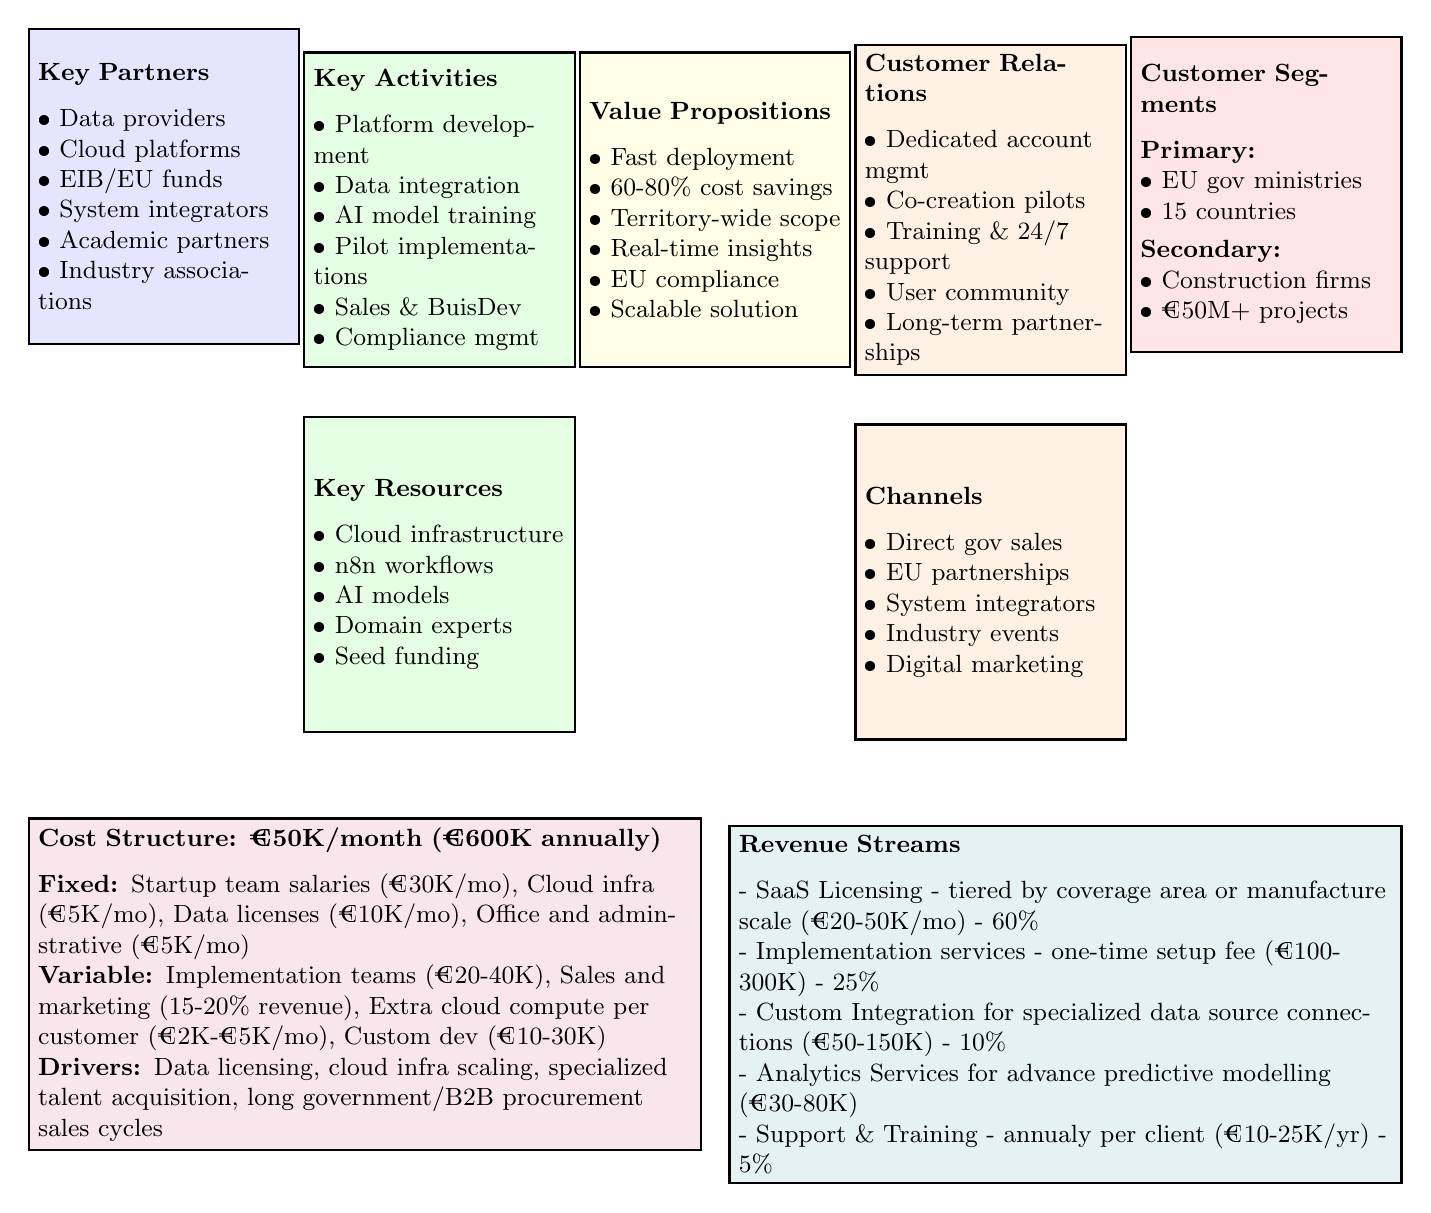
\begin{tikzpicture}[
    box/.style={rectangle, draw, thick, text width=3.2cm, minimum height=4cm, align=left, font=\small},
    tallbox/.style={rectangle, draw, thick, text width=3.2cm, minimum height=8.2cm, align=left, font=\small},
    widebox/.style={rectangle, draw, thick, text width=8.3cm, minimum height=4cm, align=left, font=\small},
    title/.style={font=\bfseries\small},
]

% Row 1 - Top boxes
\node[box, fill=blue!10] (kp) at (0,0.3) {
    \textbf{Key Partners}\\[0.2cm]
    • Data providers\\
    • Cloud platforms\\
    • EIB/EU funds\\
    • System integrators\\
    • Academic partners\\
    • Industry associations
};

\node[box, fill=green!10] (ka) at (3.5,0) {
    \textbf{Key Activities}\\[0.2cm]
    • Platform development\\
    • Data integration\\
    • AI model training\\
    • Pilot implementations\\
    • Sales \& BuisDev\\
    • Compliance mgmt
};

\node[box, fill=yellow!10] (vp) at (7,0) {
    \textbf{Value Propositions}\\[0.2cm]
    • Fast deployment\\
    • 60-80\% cost savings\\
    • Territory-wide scope\\
    • Real-time insights\\
    • EU compliance\\
    • Scalable solution
};

\node[box, fill=orange!10] (cr) at (10.5,0) {
    \textbf{Customer Relations}\\[0.2cm]
    • Dedicated account mgmt\\
    • Co-creation pilots\\
    • Training \& 24/7 support\\
    • User community\\
    • Long-term partnerships
};

\node[box, fill=red!10] (cs) at (14,0.2) {
    \textbf{Customer Segments}\\[0.2cm]
    \textbf{Primary:}\\
    • EU gov ministries\\
    • 15 countries\\[0.1cm]
    \textbf{Secondary:}\\
    • Construction firms\\
    • €50M+ projects
};

% Row 2 - Bottom boxes
\node[box, fill=green!10, below=0.6cm of ka] (kr) {
    \textbf{Key Resources}\\[0.2cm]
    • Cloud infrastructure\\
    • n8n workflows\\
    • AI models\\
    • Domain experts\\
    • Seed funding
};

\node[box, fill=orange!10, below=0.6cm of cr] (ch) {
    \textbf{Channels}\\[0.2cm]
    • Direct gov sales\\
    • EU partnerships\\
    • System integrators\\
    • Industry events\\
    • Digital marketing
};

% Row 3 - Wide bottom boxes
\node[widebox, fill=purple!10, below=6.0cm of kp.south west, anchor=north west] (cost) {
    \textbf{Cost Structure: €50K/month (€600K annually)}\\[0.2cm]
    \textbf{Fixed:} Startup team salaries (€30K/mo), Cloud infra (€5K/mo), Data licenses (€10K/mo), Office and adminstrative (€5K/mo)\\
    \textbf{Variable:} Implementation teams (€20-40K), Sales and marketing (15-20\% revenue), Extra cloud compute per customer (€2K-€5K/mo), Custom dev (€10-30K)\\
    \textbf{Drivers:} Data licensing, cloud infra scaling, specialized talent acquisition, long government/B2B procurement sales cycles
};

\node[widebox, fill=teal!10, below=6.0cm of cs.south east, anchor=north east] (revenue) {
    \textbf{Revenue Streams}\\[0.2cm]
    - SaaS Licensing - tiered by coverage area or manufacture scale (€20-50K/mo) - 60\%\\
    - Implementation services - one-time setup fee (€100-300K) - 25\%\\
    - Custom Integration for specialized data source connections (€50-150K) - 10\%\\
    - Analytics Services for advance predictive modelling (€30-80K)\\
    - Support \& Training - annualy per client (€10-25K/yr) - 5\%
};

\end{tikzpicture}
}
\caption{TerraSync AI Business Model Canvas}
\end{figure}

\subsubsection{Customer Segments}
\textbf{Primary segment:} EU Government Ministries responsible for infrastructure, transport, environment, and regional development in 15 countries with GNI below 90\% EU average, requiring EU Green Deal compliance and resource optimization tools.

\textbf{Secondary segment:} Large construction and engineering firms (€50M+ projects) operating in target regions, needing EU compliance documentation and project optimization capabilities.

\subsubsection{Value Propositions}
Our platform delivers rapid deployment in weeks rather than years, offering 60-80\% cost savings compared to custom digital twin development by leveraging orchestration of existing tools rather than reinventing infrastructure. We provide real-time actionable insights beyond simple visualization, automated EU Green Deal sustainability reporting, and scalable implementation from pilot to country-wide coverage in months.

\subsubsection{Channels}
We reach customers through direct government procurement processes, EU partnership programs including EIB financing packages and Cohesion Fund applications, strategic alliances with system integrators like Accenture and Deloitte, presence at EU infrastructure summits and smart city conferences, and targeted digital marketing via LinkedIn, industry publications, and published case studies.

\subsubsection{Customer Relationships}
We maintain dedicated account management for government clients, co-create solutions through pilot projects with early adopters, provide comprehensive training and support including on-site workshops, documentation, and 24/7 helpdesk services, foster user communities for best practice sharing, and establish long-term partnerships through multi-year contracts with expansion clauses.

\textbf{Projected Revenue Mix (Year 3):}
SaaS licensing accounts for 60\% of revenue, implementation services 25\%, custom integration and analytics 10\%, and support and training 5\%.

\subsubsection{Key Resources}
Our physical resources include cloud infrastructure on AWS/Azure, development workstations, and demo environments. Intellectual assets comprise proprietary n8n workflow templates, AI models for infrastructure prediction, data processing pipelines, and our unique territory-wide orchestration methodology. Human capital includes data scientists, ML engineers, n8n specialists, infrastructure domain experts, sales teams, and support engineers. Financial resources encompass €500K-1M seed funding, data licensing agreements, and EIB co-investment arrangements.

\subsubsection{Key Activities}
Core activities include platform development and maintenance, data source integration and workflow orchestration, AI model training and continuous improvement, customer pilot implementations, sales and business development, compliance and security management, and ongoing research and innovation for continuous improvement.

\subsubsection{Key Partnerships}
Strategic partnerships span data providers including weather services, satellite imagery providers like Copernicus, and GIS databases; technology partners such as Azure, AWS, and the n8n community; funding partners including the European Investment Bank and EU Cohesion Fund administrators; system integrators like Accenture, Deloitte, and local consulting firms; academic partners for AI model development; and industry associations including EU construction federations and smart city alliances.

\newpage

% ---------------------------
% 6. DIGITAL TOOLS INTEGRATION
% ---------------------------
\section{Digital Tools Integration}

\subsection{Technology Stack Overview}

\begin{table}[H]
\centering
\caption{Comprehensive Technology Stack}
\small
\begin{tabular}{@{}p{0.2\textwidth}p{0.25\textwidth}p{0.2\textwidth}p{0.25\textwidth}@{}}
\toprule
\textbf{Category} & \textbf{Tool/Technology} & \textbf{Purpose} & \textbf{Rationale} \\ \midrule
Orchestration & n8n & Workflow automation & Open-source, flexible, cost-effective \\
Data Ingestion & Apache Kafka & High-volume streaming & Handles IoT sensor loads \\
AI/ML & Azure ML + TensorFlow & Pattern recognition & Pre-trained + custom models \\
Storage & TimescaleDB & Time-series data & Optimized for simulation histories \\
Visualization & Grafana + Custom React & Real-time dashboards & Stakeholder-friendly \\
Digital Twin 3D & Unity/Unreal Engine & Territory simulation & Visual representation \\
GIS Processing & PostGIS + QGIS & Geospatial analysis & Industry standard \\
API Management & Kong Gateway & API orchestration & Security, rate limiting \\
Monitoring & Prometheus + Grafana & System monitoring & Real-time performance \\
DevOps & Docker + Kubernetes & Container orchestration & Scalability \\
\bottomrule
\end{tabular}
\end{table}

\subsection{Core Platform Components}

\subsubsection{n8n Orchestration Hub}
\textbf{Why n8n is central to our competitive advantage:}
\begin{itemize}
    \item \textbf{Visual Workflow Design:} Non-developers can create integrations
    \item \textbf{400+ Pre-built Connectors:} APIs, databases, webhooks
    \item \textbf{Custom Code Execution:} Python, JavaScript for specialized logic
    \item \textbf{Self-hosted:} Data sovereignty compliance
    \item \textbf{Cost:} Open-source vs. \$10K-50K/month for enterprise iPaaS
\end{itemize}

\textbf{Example Workflows:}
\begin{enumerate}
    \item Weather API → Process → Update territory risk scores → Alert stakeholders
    \item Satellite imagery → Object detection AI → Infrastructure change detection → Report
    \item IoT sensors → Anomaly detection → Predictive maintenance alert → Work order
\end{enumerate}

\subsubsection{AI/ML Pipeline}
\begin{itemize}
    \item \textbf{Data Preprocessing:} Clean, normalize, and aggregate multi-source data
    \item \textbf{Feature Engineering:} Extract predictive variables (weather patterns, traffic flows, construction activity)
    \item \textbf{Model Types:}
    \begin{itemize}
        \item Time-series forecasting (LSTM, Prophet)
        \item Computer vision (YOLOv8 for satellite imagery)
        \item Anomaly detection (Isolation Forest)
        \item Optimization algorithms (genetic algorithms for resource allocation)
    \end{itemize}
    \item \textbf{Continuous Learning:} Models retrain monthly on new data
\end{itemize}

\subsubsection{Digital Twin Rendering}
\begin{itemize}
    \item \textbf{Unity 3D Engine:} Real-time territory visualization
    \item \textbf{LOD (Level of Detail):} Optimize rendering for large areas
    \item \textbf{Data Layers:} Toggle infrastructure, weather, traffic, pollution
    \item \textbf{Temporal Controls:} Playback historical data, simulate future scenarios
\end{itemize}

\subsection{Scalability and Performance}

\textbf{Current Capacity:}
\begin{itemize}
    \item Process 1M+ data points per day
    \item Support 5-10 concurrent territories
    \item Sub-second dashboard updates
\end{itemize}

\textbf{Scaling Strategy:}
\begin{itemize}
    \item Kubernetes horizontal auto-scaling
    \item CDN for global dashboard access
    \item Database sharding by territory
    \item Multi-region cloud deployment
\end{itemize}

\subsection{Security and Compliance}

\textbf{Data Security:}
\begin{itemize}
    \item End-to-end encryption (TLS 1.3)
    \item Role-based access control (RBAC)
    \item Data anonymization for sensitive information
    \item SOC 2 Type II compliance roadmap
\end{itemize}

\textbf{GDPR Compliance:}
\begin{itemize}
    \item Data minimization principles
    \item Right to erasure implementation
    \item Data Processing Agreements with partners
    \item EU data residency (servers in Frankfurt/Dublin)
\end{itemize}

\subsection{Integration Roadmap}

\textbf{Phase 1 (Months 1-6): MVP}
\begin{itemize}
    \item 5 core data sources
    \item Basic n8n workflows
    \item Single territory support (Cyprus)
    \item 2D dashboard
\end{itemize}

\textbf{Phase 2 (Months 7-12): Enhanced}
\begin{itemize}
    \item 15+ data sources
    \item Advanced AI models
    \item Multi-territory support (3 countries)
    \item 3D visualization
\end{itemize}

\textbf{Phase 3 (Year 2): Enterprise}
\begin{itemize}
    \item 30+ data sources
    \item White-label capabilities
    \item Mobile applications
    \item API marketplace for third-party extensions
\end{itemize}

\newpage

% ---------------------------
% 7. SCENARIO-BASED PLANNING
% ---------------------------
\section{Scenario-Based Planning}

\subsection{Scenario 1: Best Case - "Rapid Adoption"}

\textbf{Key Assumptions:}
\begin{itemize}
    \item Cyprus pilot succeeds within 6 months
    \item EU Green Deal enforcement accelerates
    \item 2 additional governments sign by Month 12
    \item Positive media coverage and case studies
\end{itemize}

\textbf{Strategic Response:}
\begin{itemize}
    \item Accelerate hiring (10 employees by Year 2)
    \item Expand to 5 Balkan countries
    \item Raise Series A funding (€5M)
    \item Develop white-label product
\end{itemize}

\textbf{Financial Projections:}
\begin{itemize}
    \item Year 1: €800K revenue
    \item Year 2: €2.5M revenue
    \item Year 3: €6M revenue
    \item Break-even: Month 14
\end{itemize}

\subsection{Scenario 2: Most Likely - "Steady Growth"}

\textbf{Key Assumptions:}
\begin{itemize}
    \item Cyprus pilot takes 9-12 months
    \item Long government sales cycles (18 months average)
    \item 1 new government client per year
    \item Competition from established players
\end{itemize}

\textbf{Strategic Response:}
\begin{itemize}
    \item Focus on 2-3 core markets
    \item Controlled team growth (5-7 employees by Year 2)
    \item Pursue EIB co-investment arrangements
    \item Develop strong customer success function
\end{itemize}

\textbf{Financial Projections:}
\begin{itemize}
    \item Year 1: €500K revenue
    \item Year 2: €1.5M revenue
    \item Year 3: €4M revenue
    \item Break-even: Month 18
\end{itemize}

\subsection{Scenario 3: Worst Case - "Slow Traction"}

\textbf{Key Assumptions:}
\begin{itemize}
    \item Cyprus pilot delayed (12-18 months)
    \item Budget cuts due to economic recession
    \item Data access restrictions
    \item Longer proof-of-concept requirements
\end{itemize}

\textbf{Strategic Response:}
\begin{itemize}
    \item Pivot to enterprise customers (construction firms)
    \item Reduce burn rate (lean team of 3-4)
    \item Develop smaller-scope products (single use-case tools)
    \item Extend runway with consulting services
\end{itemize}

\textbf{Financial Projections:}
\begin{itemize}
    \item Year 1: €200K revenue
    \item Year 2: €600K revenue
    \item Year 3: €1.8M revenue
    \item Break-even: Month 30+
\end{itemize}

\subsection{Strategic Adaptability}

\textbf{Early Warning Indicators:}
\begin{itemize}
    \item Month 6: If no signed pilot MOU, activate secondary market strategy
    \item Month 12: If < €300K revenue, implement cost reduction plan
    \item Month 18: If < 2 paying customers, consider pivot or strategic acquisition
\end{itemize}

\textbf{Contingency Plans:}
\begin{itemize}
    \item Product pivot to white-label for consulting firms
    \item Geographic pivot to higher-growth markets (Asia-Pacific)
    \item Feature pivot to specialized tools (e.g., maritime-only)
    \item Strategic partnership with established digital twin vendor
\end{itemize}

\newpage

% ---------------------------
% 8. IMPLEMENTATION ROADMAP & FINANCIAL OVERVIEW
% ---------------------------
\section{Implementation Roadmap \& Financial Overview}

\subsection{Phased Implementation Plan}

\subsubsection{Phase 1: Foundation (Months 1-6)}
\textbf{Objectives:} Build MVP, secure pilot customer, establish partnerships

\begin{table}[H]
\centering
\caption{Phase 1 Milestones}
\small
\begin{tabular}{@{}p{0.15\textwidth}p{0.35\textwidth}p{0.2\textwidth}p{0.2\textwidth}@{}}
\toprule
\textbf{Month} & \textbf{Key Activities} & \textbf{Deliverables} & \textbf{Investment} \\ \midrule
1-2 & Team formation, legal setup, partnership outreach & Company registered, 3 core team members & €50K \\
3-4 & MVP development, data source integration & n8n workflows, 5 data sources connected & €80K \\
5-6 & Cyprus pilot negotiation, implementation begins & Signed MOU, pilot deployment & €70K \\ \bottomrule
\end{tabular}
\end{table}

\subsubsection{Phase 2: Validation (Months 7-12)}
\textbf{Objectives:} Deliver pilot results, expand to 2-3 territories

\begin{table}[H]
\centering
\caption{Phase 2 Milestones}
\small
\begin{tabular}{@{}p{0.15\textwidth}p{0.35\textwidth}p{0.2\textwidth}p{0.2\textwidth}@{}}
\toprule
\textbf{Month} & \textbf{Key Activities} & \textbf{Deliverables} & \textbf{Investment} \\ \midrule
7-9 & Cyprus pilot execution, results analysis & Pilot report, case study & €90K \\
10-12 & Sales to 2 additional governments, product enhancement & 2 new contracts, v2.0 launch & €120K \\ \bottomrule
\end{tabular}
\end{table}

\subsubsection{Phase 3: Expansion (Year 2)}
\textbf{Objectives:} Scale to 6+ territories, expand team, achieve profitability

\begin{itemize}
    \item Q1: Add 2 Balkan countries (Montenegro, North Macedonia)
    \item Q2: Launch 3D visualization, expand data sources to 20+
    \item Q3: Add Baltic states (Latvia, Estonia)
    \item Q4: Achieve operational profitability, prepare Series A
\end{itemize}

\subsection{Financial Projections}

\subsubsection{Revenue Forecast (Most Likely Scenario)}

\begin{table}[H]
\centering
\caption{3-Year Revenue Projections (€K)}
\begin{tabular}{@{}lcccc@{}}
\toprule
\textbf{Revenue Stream} & \textbf{Year 1} & \textbf{Year 2} & \textbf{Year 3} \\ \midrule
SaaS Subscriptions & 240 & 900 & 2,400 \\
Implementation Services & 150 & 400 & 1,000 \\
Custom Integration & 80 & 150 & 400 \\
Support \& Training & 30 & 50 & 200 \\ \midrule
\textbf{Total Revenue} & \textbf{500} & \textbf{1,500} & \textbf{4,000} \\ \bottomrule
\end{tabular}
\end{table}

\subsubsection{Cost Structure}

\begin{table}[H]
\centering
\caption{3-Year Operating Costs (€K)}
\begin{tabular}{@{}lcccc@{}}
\toprule
\textbf{Cost Category} & \textbf{Year 1} & \textbf{Year 2} & \textbf{Year 3} \\ \midrule
Personnel (3→5→8 employees) & 360 & 600 & 960 \\
Cloud Infrastructure & 60 & 120 & 240 \\
Data Licenses & 120 & 180 & 300 \\
Sales \& Marketing & 100 & 225 & 600 \\
Office \& Admin & 60 & 100 & 150 \\
R\&D & 80 & 150 & 250 \\ \midrule
\textbf{Total Operating Costs} & \textbf{780} & \textbf{1,375} & \textbf{2,500} \\ \bottomrule
\end{tabular}
\end{table}

\subsubsection{Cash Flow and Funding Requirements}

\begin{table}[H]
\centering
\caption{3-Year Cash Flow Summary (€K)}
\begin{tabular}{@{}lccc@{}}
\toprule
& \textbf{Year 1} & \textbf{Year 2} & \textbf{Year 3} \\ \midrule
Revenue & 500 & 1,500 & 4,000 \\
Operating Costs & (780) & (1,375) & (2,500) \\
\textbf{EBITDA} & \textbf{(280)} & \textbf{125} & \textbf{1,500} \\ \midrule
Cumulative Cash Flow & (280) & (155) & 1,345 \\
\bottomrule
\end{tabular}
\end{table}

\textbf{Funding Strategy:}
\begin{itemize}
    \item \textbf{Seed Round (Month 0):} €500K (angels, early-stage VCs)
    \item \textbf{EIB Co-investment (Month 12):} €300K (tied to government contracts)
    \item \textbf{Series A (Month 24):} €3-5M (growth capital for expansion)
\end{itemize}

\textbf{Use of Funds (Seed):}
\begin{itemize}
    \item Product development: 40\% (€200K)
    \item Sales \& pilot implementation: 30\% (€150K)
    \item Operations \& team: 20\% (€100K)
    \item Reserve: 10\% (€50K)
\end{itemize}

\subsection{Key Financial Metrics}

\begin{table}[H]
\centering
\caption{Unit Economics \& Key Metrics}
\begin{tabular}{@{}lc@{}}
\toprule
\textbf{Metric} & \textbf{Value} \\ \midrule
Customer Acquisition Cost (CAC) & €80K \\
Lifetime Value (LTV) & €450K (3 years) \\
LTV:CAC Ratio & 5.6:1 \\
Gross Margin & 65\% \\
Payback Period & 14 months \\
Churn Rate (Annual) & <5\% (gov contracts) \\ \bottomrule
\end{tabular}
\end{table}

\subsection{Risk Mitigation}

\textbf{Financial Risks:}
\begin{itemize}
    \item \textbf{Long sales cycles:} Mitigate with pipeline of 3-5x target customers
    \item \textbf{Data licensing costs:} Negotiate volume discounts, use open data
    \item \textbf{Currency fluctuations:} Price in EUR, hedge where necessary
\end{itemize}

\textbf{Operational Risks:}
\begin{itemize}
    \item \textbf{Talent acquisition:} Remote-first model, competitive comp
    \item \textbf{Data quality:} Automated validation, partner SLAs
    \item \textbf{Technical complexity:} Modular architecture, strong documentation
\end{itemize}

\newpage

% ---------------------------
% 9. CONCLUSION & REFLECTION
% ---------------------------
\section{Conclusion \& Reflection}

\subsection{Key Takeaways}

TerraSync AI addresses a validated market need at the intersection of three powerful trends:
\begin{enumerate}
    \item \textbf{EU Green Deal Mandates:} Legal requirements for sustainability create non-discretionary demand
    \item \textbf{Infrastructure Crisis:} 20-30\% waste in \$57 trillion global spending creates massive savings opportunity
    \item \textbf{Digital Twin Adoption:} 40\%+ market CAGR demonstrates technology maturity and acceptance
\end{enumerate}

Our competitive advantage lies not in reinventing digital twin technology, but in our unique **orchestration approach**:
\begin{itemize}
    \item n8n-based integration enables rapid deployment (weeks vs. years)
    \item Territory-wide scope vs. project-specific competitors
    \item Cost-effective for resource-constrained governments (60-80\% cheaper)
    \item Open architecture supports continuous innovation
\end{itemize}

\subsection{Venture Potential}

\textbf{Market Opportunity:}
\begin{itemize}
    \item TAM: €259B digital twin market by 2032
    \item SAM: €8-12B (infrastructure-focused, target regions)
    \item SOM: €100-150M (3-5\% market share in target segments by Year 5)
\end{itemize}

\textbf{Success Factors:}
\begin{itemize}
    \item Early customer validation (Cyprus pilot)
    \item Strong partnerships (EIB, data providers)
    \item Lean operations with high leverage (orchestration vs. custom builds)
    \item Network effects from data aggregation
\end{itemize}

\textbf{Exit Opportunities:}
\begin{itemize}
    \item Strategic acquisition by established players (Siemens, Bentley, Autodesk)
    \item Vertical integration by consulting firms (Accenture, Deloitte)
    \item Public markets (5-7 year horizon)
\end{itemize}

\subsection{Lessons Learned Through This Process}

\textbf{1. Problem Validation is Critical}
\begin{itemize}
    \item Initial web research confirmed 20-30\% waste in construction/infrastructure
    \item McKinsey data validated productivity decline and massive spending needs
    \item EU regulatory mandates create urgency beyond cost savings alone
\end{itemize}

\textbf{2. Business Model Must Match Customer Reality}
\begin{itemize}
    \item Long government sales cycles require patient capital and pipeline depth
    \item SaaS pricing must reflect value delivered (cost savings) not just cost-plus
    \item Implementation services crucial for adoption but can't dominate revenue mix
\end{itemize}

\textbf{3. Technology is Enabler, Not Differentiator}
\begin{itemize}
    \item n8n orchestration is key, but must be invisible to customers
    \item AI/ML models require continuous validation against customer KPIs
    \item "Territory-wide" scope is strategic differentiator, not technology choice
\end{itemize}

\textbf{4. Scenario Planning Reduces Risk}
\begin{itemize}
    \item Best/likely/worst case scenarios force hard questions about assumptions
    \item Early warning indicators enable proactive adaptation
    \item Contingency plans (pivot options) reduce founder anxiety and investor risk
\end{itemize}

\subsection{Personal Reflection}

\textit{[Placeholder: Add 150-200 words reflecting on:
\begin{itemize}
    \item What you learned about digital entrepreneurship
    \item Challenges faced in developing this plan
    \item How your thinking evolved through the research process
    \item Skills you developed (market analysis, business model design, etc.)
    \item What you would do differently with more time/resources
\end{itemize}
]}

\subsection{Next Steps}

\textbf{Immediate Actions (Next 30 Days):}
\begin{enumerate}
    \item Conduct 5 customer discovery interviews with Cyprus government officials
    \item Build working n8n prototype with 3 data sources
    \item Submit EU Cohesion Fund pre-application
    \item Recruit technical co-founder (data science background)
\end{enumerate}

\textbf{Short-term Goals (3-6 Months):}
\begin{enumerate}
    \item Secure seed funding (€500K)
    \item Sign Cyprus pilot MOU
    \item Establish data partnerships (weather, satellite imagery)
    \item Build MVP v1.0
\end{enumerate}

\textbf{Long-term Vision:}
TerraSync AI will become the de facto standard for territory-wide infrastructure optimization in emerging EU economies, reducing waste, accelerating sustainable development, and demonstrating that smart orchestration of existing tools can outperform expensive custom solutions.

\newpage
\printbibliography
\nocite{*}

\end{document}
